\documentclass[a4paper,10pt]{article}
%\documentclass[a4paper,10pt]{scrartcl}

\usepackage[utf8]{inputenc}
\usepackage{amsmath}
\usepackage{graphicx}

\title{HW-4}
\author{Chi Zhang}
\date{14/10/2015}

\pdfinfo{%
  /Title    (HW-4)
  /Author   (Chi Zhang)
  /Creator  ()
  /Producer ()
  /Subject  ()
  /Keywords (VLSI, EL-6473, Homework)
}

\begin{document}
\maketitle
\section*{Problem 1}
\begin{figure}
 \centering
 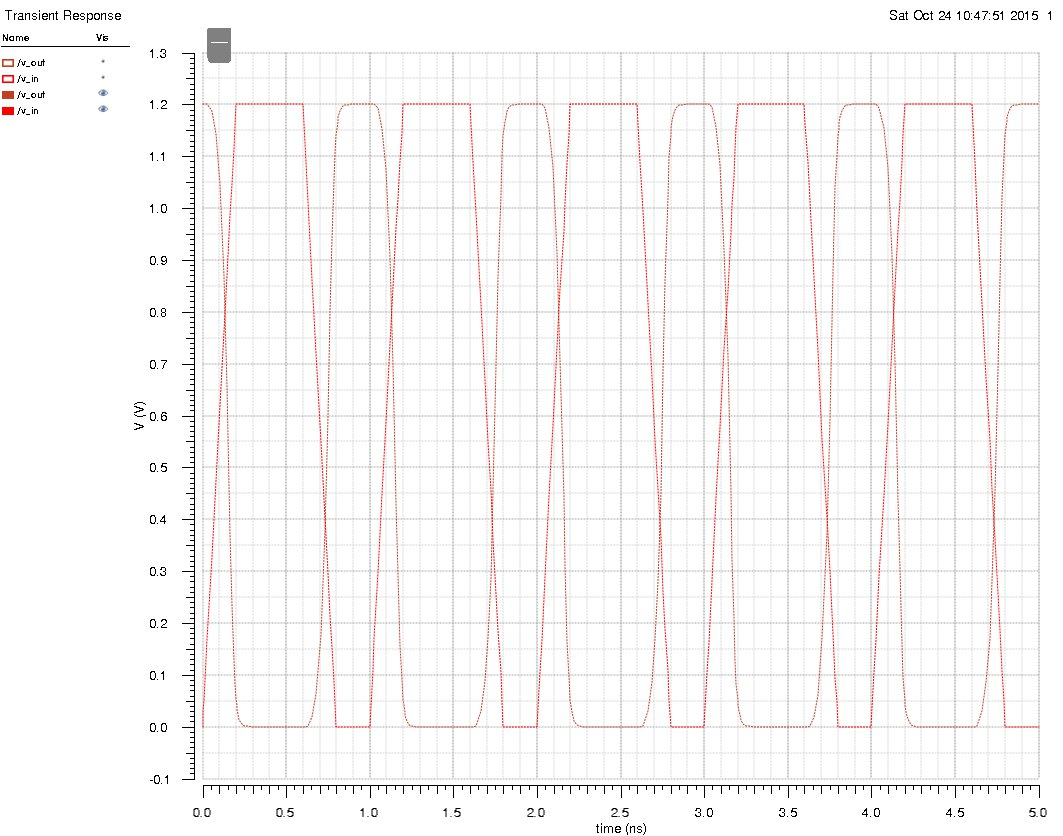
\includegraphics[width=10cm]{HW4_Q1.jpg}
 \caption{Q1}
\end{figure}
\begin{math}r = \frac{135.75}{90}\end{math}. \begin{math}t_{pLH} = t_{pHL} = 0.05ns\end{math}.\\
\\
Please see Figure 1 for Candence simulation result.
\section*{Problem 2}
\subsection*{a}
\begin{figure}
 \centering
 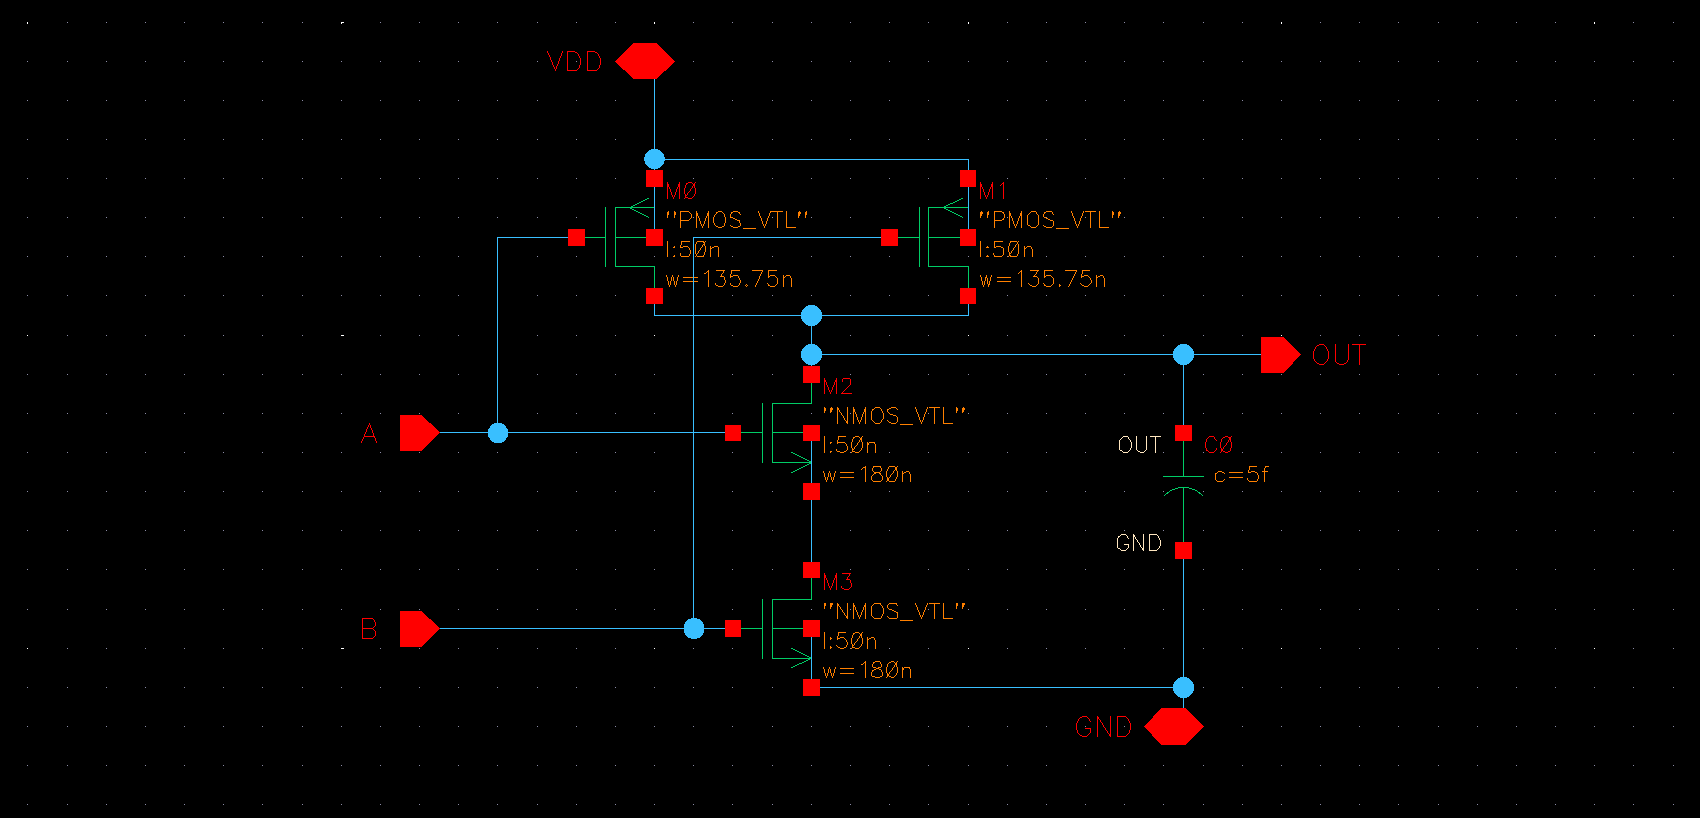
\includegraphics[width=10cm]{NAND2.png}
 \caption{Q2.a: NAND2 schematic}
\end{figure}
\begin{figure}
 \centering
 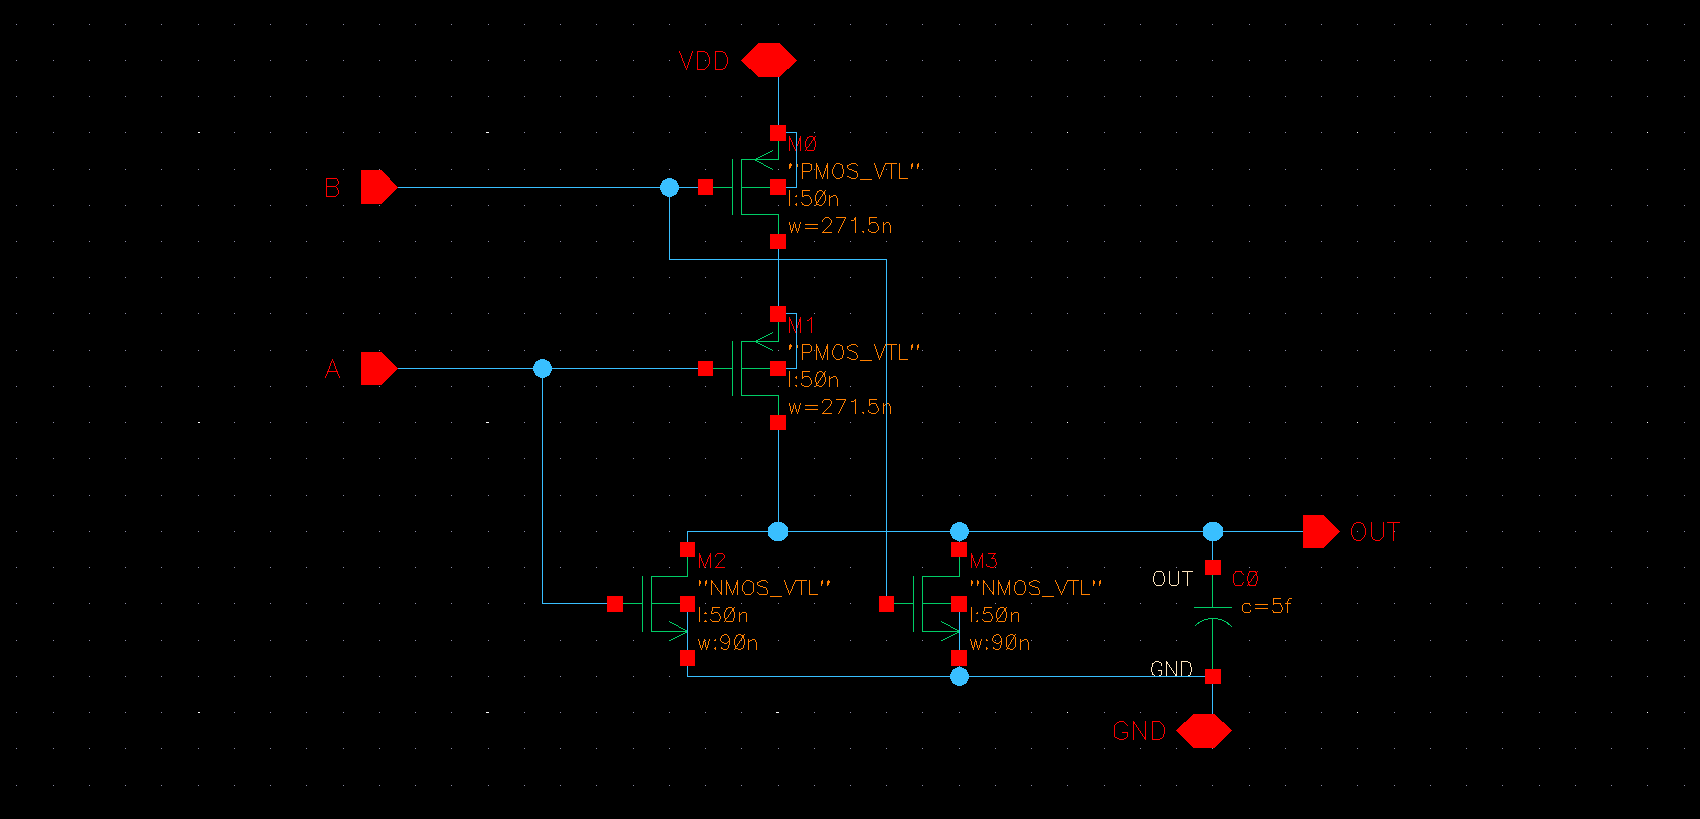
\includegraphics[width=10cm]{NOR2.png}
 \caption{Q2.a: NOR2 schematic}
\end{figure}
Please see Figure 2 for NAND2 schematic, and Figure 3 for NOR2 schematic.
\subsection*{b}
Please see Figure 4 to 7 for simulation results.\\
\begin{tabular}{|c|c|c|c|}
 \hline
 Gate & Input Pattern & \begin{math}t_{pLH}\end{math} & \begin{math}t_{pHL}\end{math}\\ \hline
 NAND2& A = 1, B pulse&84 ps&48 ps\\ \cline{2-4}
 &A pulse, B = 1&81 ps&59 ps\\ \hline
 NOR2& A = 0, B pulse&52 ps&83 ps\\ \cline{2-4}
 &A pulse, B = 0&61 ps&80 ps\\ \hline
\end{tabular}
\begin{figure}
 \centering
 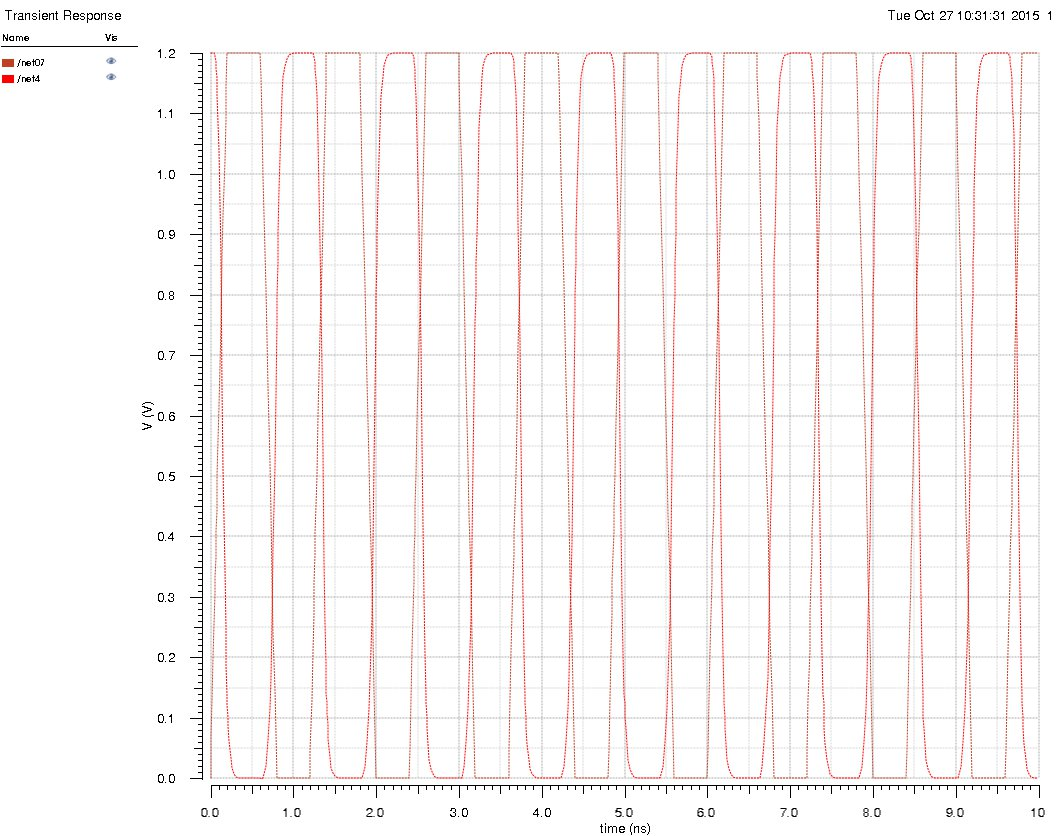
\includegraphics[width=10cm]{HW4_Q2_b_NAND2_B_pulse.jpg}
 \caption{Q2.b: NAND2: A = 1, B pulse.}
\end{figure}
\begin{figure}
 \centering
 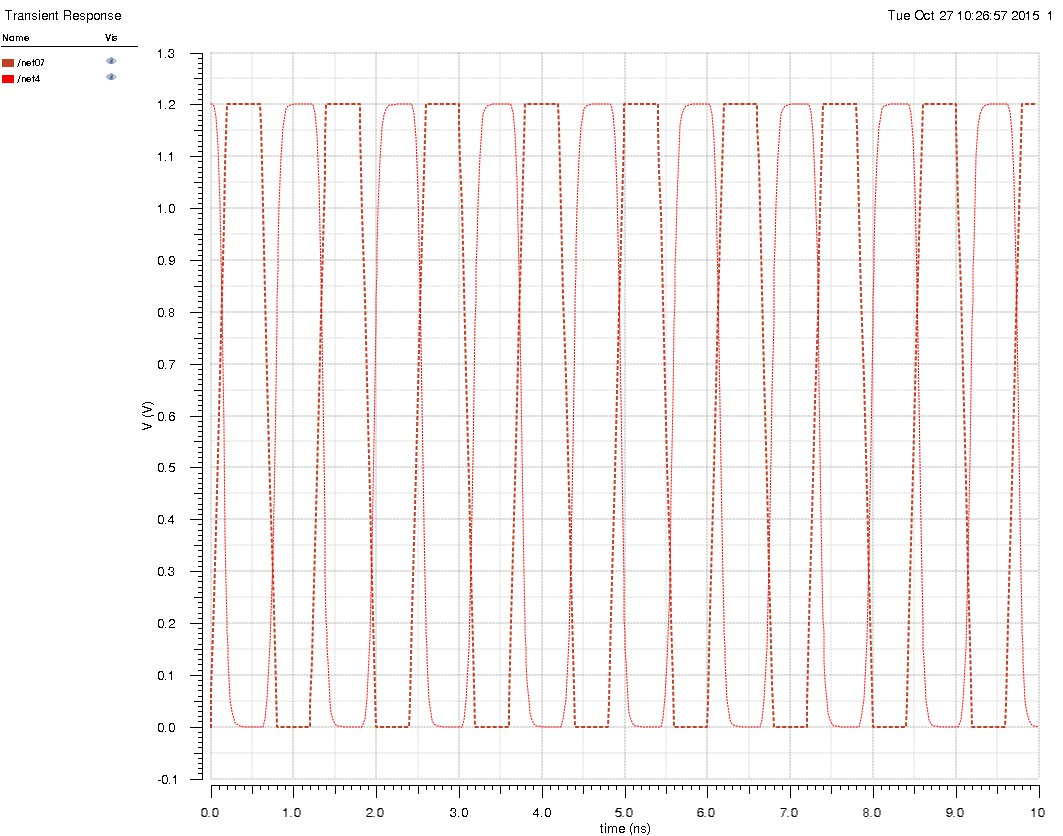
\includegraphics[width=10cm]{HW4_Q2_b_NAND2_A_pulse.jpg}
 \caption{Q2.b: NAND2: A pulse, B = 1.}
\end{figure}
\begin{figure}
 \centering
 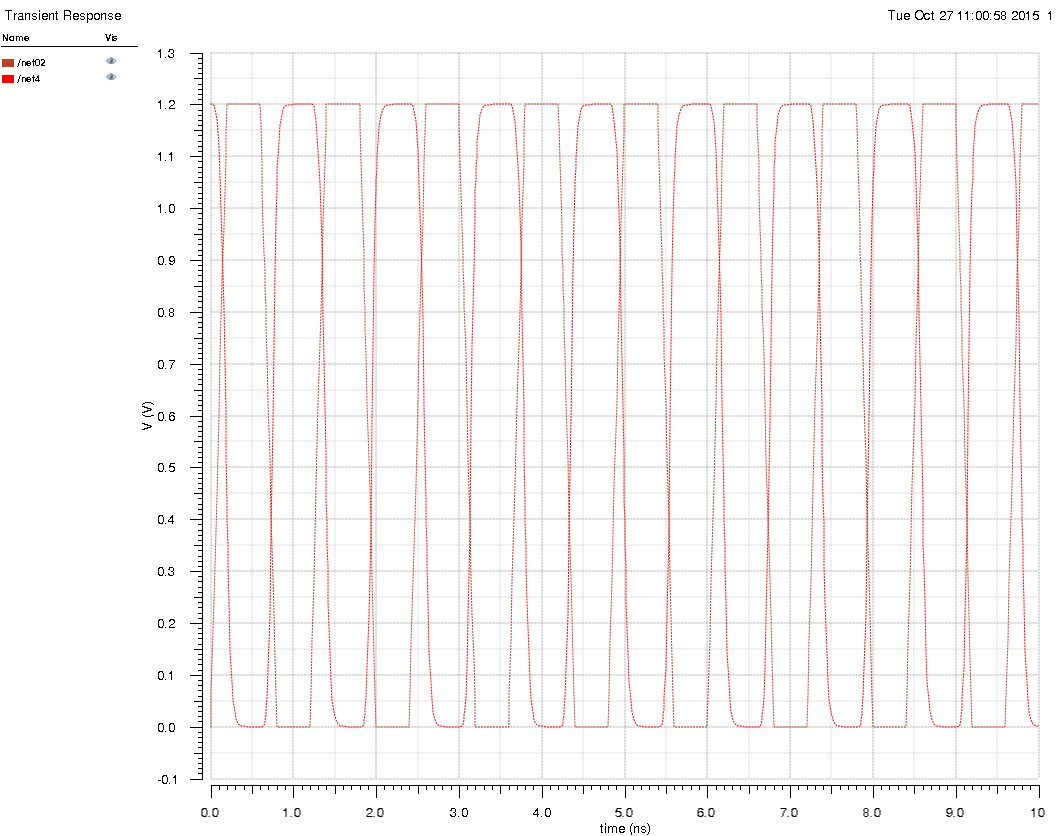
\includegraphics[width=10cm]{HW4_Q2_b_NOR2_B_pulse.jpg}
 \caption{Q2.b: NOR2: A = 0, B pulse.}
\end{figure}
\begin{figure}
 \centering
 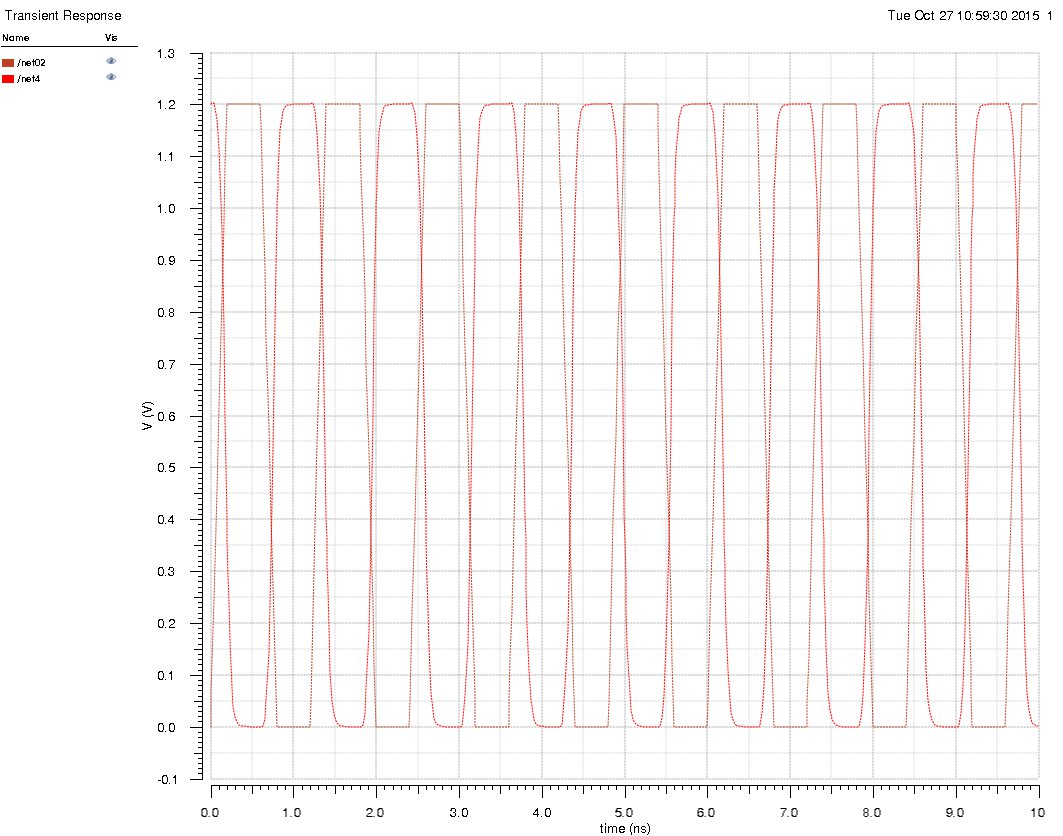
\includegraphics[width=10cm]{HW4_Q2_b_NOR2_A_pulse.jpg}
 \caption{Q2.b: NOR2: A pulse, B = 0.}
\end{figure}
\subsection*{c}
For NAND2, input pattern A = 1, B is 0 to 1 has the worst low-to-high delay; input pattern A is 1 to 0, B = 1 has the worst 
high-to-low delay.\\
\\
For NOR2, input pattern A = 0, B is 1 to 0 has the worst high-to-low delay; input pattern A is 0 to 1, B = 0 has the worst
low-to high delay.
\subsection*{d}
\begin{tabular}{|c|c|c|}
 \hline
 Gate&Input Pattern&Propogation delay p\\ \hline
 NAND2& A = 1, B pulse&66 ps\\ \cline{2-3}
 &A pulse, B = 1&70 ps\\ \hline
 NOR2& A = 0, B pulse&67.5 ps\\ \cline{2-3}
 &A pulse, B = 0&70.5 ps\\ \hline
\end{tabular}
\\
\\
Evidently, there is defferences as for propogation delay related to input pattern.
\section*{Problem 3}
\subsection*{a}
\begin{math}t_{pLH}\end{math} for \begin{math}C_a\end{math} should equals to \begin{math}t_{pLH}\end{math} for
\begin{math}C_L\end{math}, hence,
\begin{equation}
\begin{split}
 R_n & C_a ln(\frac{1}{1-\frac{\Delta V_a}{V_{DD} - V_{Tn}}}) = R_n C_L ln(\frac{1}{1-\frac{\Delta V_{out}}{V_{DD}}})\\
 \frac{C_a}{C_L} &= \frac{ln(\frac{1}{1-\frac{\Delta V_{out}}{V_{DD}}})}{ln(\frac{1}{1-\frac{\Delta V_a}{V_{DD} - V_{Tn}}})}
\end{split}
\end{equation}
For \begin{math}\Delta V_{out} = 0.6V\end{math}, \begin{math}\Delta V_a = 1.4V\end{math}, thus 
\begin{math}\frac{C_a}{C_L} = 0.2279\end{math}.\\
For \begin{math}\Delta V_{out} = 0.8V\end{math}, \begin{math}\Delta V_a = 1.2V\end{math}, thus 
\begin{math}\frac{C_a}{C_L} = 0.4209\end{math}.\\
Thus, \begin{math}0.2279 \leq \frac{C_a}{C_L} \leq 0.4209\end{math}.
\subsection*{b}
For (i) A = 0, B = 0 to 1:\\
\begin{math}C_a\end{math} is charged in precharge phase. Thus both \begin{math}C_L\end{math} and \begin{math}C_a\end{math}
 need to be discharged in evaluation phase.\\
For (ii) B = 1, A = 0 to 1:\\
Only \begin{math}C_L\end{math} is charged in precharge phase. Thus only \begin{math}C_L\end{math} needs to be discharged in 
evaluation phase.\\
Thus, case (ii) results in the lower high-to-low delay.
\end{document}
